\section{Pla d'acció}
\subsection{Diagrama de Gantt}
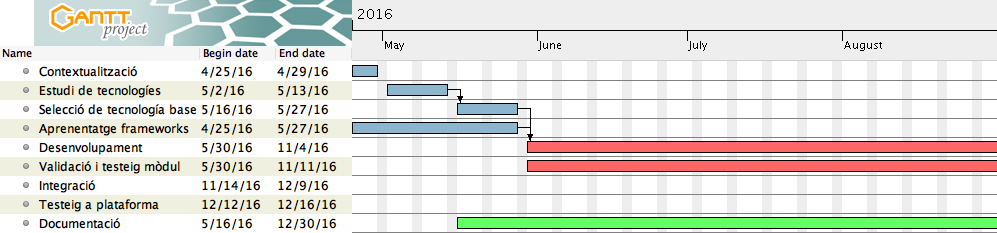
\includegraphics[scale=0.5]{img/ganttHPart1.png}	
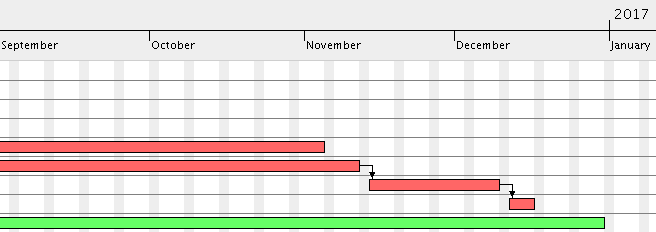
\includegraphics[scale=0.5]{img/ganttHPart2.png}	

\subsection{Interpretació}
Com es pot apreciar al diagrama anterior, la planificació està prevista per a que el projecte, començant juntament amb el conveni el 25 d'abril d'aquest mateix any, finalitzi en acabar l'any.\\
\newline Dins del projecte, tal i com es pot haver apreciat durant l'explicació de les tasques, podem trobar tres fases clarament diferenciades.
\renewcommand{\labelenumi}{\roman{enumi}}
\begin{enumerate}
	\item En aquesta primera part, marcada en el diagrama de gantt anterior amb color blau, es pretén assentar les bases per al posterior desenvolupament, adquirir tots, o si més no gran part,  els coneixements necessaris per a dur a bon port el futur desenvolupament.\\
		\newline En aquesta primera fase s'inclou, la lectura i anàlisi de les diferents lleis sobre signatura, investigació sobre possibles tencologies i camins a seguir, així com agafar una mica de rodatge amb les tecnologies emprades dins de la pròpia empresa.
	\item Seguidament, marcada a la figura anterior de color vermell, el gruix del projecte. Tot el desenvolupament on s'han d'aplicar tots els coneixements adquirits durant el transcurs de la fase anterior.\\
		\newline Aquesta fase inclou tot el procés de desenvolupament i testeig del mòdul, així com la seva posterior integració a la plataforma i el seu corresponent testeig.
	\item Finalment, es pot apreciar de color verd, a la figura anterior, una fase que comença a mitjans de la fase de cerca: el procés de documentació.\\
		\newline És important que es documenti a mesura que es desenvolupa per tal del mantenir la informació al dia, i que en un futur, la informació enmagatzemada dins d'aquesta documentació no sigui fruit del record del moment sobre una decisió concreta.
\end{enumerate}

\subsection{Desviacions}
Com en tot projecte, existeix la possibilitat de que sorgeixin desviacions que fan que els temps pensats inicialment no es compleixin.\\
Per pal·liar aquestes possibles desviacions, es contemplen tres possibles accions inicials:
\begin{itemize}
	\item \textbf{Ampliació de l'equip de desenvolupament}\\
Aquesta opció, tal i com indica el seu nom, consisteix en la contractació de nous desenvolupadors, ja sigui amb un caràcter definitiu o temporal, per tal de reforçar l'equip i permetre assolir les diferents tasques que formen el projecte més ràpidament i amb una major solvència.\\
	\item \textbf{Aplaçar la data final de lliurament}\\
Al tractar-se d'un Treball de Final de Grau, la data d'entrega queda estipulada des d'un primer moment amb la intenció de fitar el projecte dins del quadrimestre corresponent; per altra banda, la finalització del conveni amb l'empresa també dictamina una data límit.\\
	\item \textbf{Reformular els requisits del projecte}\\
Finalment, la última opció que es planteja consisteix en reformular el plantejament inicial del que hauria de ser el projecte acabat, amb la idea d'eliminar aquelles \textit{features} que no siguin estrictament necessàries i vitals per al bon funcionament d'aquest i que no siguin claus per a la seva posterior integració amb la plataforma.\\
\end{itemize}
De totes les opcions presentades, la que sembla que més viabilitat té dins dels plantejament que es dóna al projecte és la tecera, que planteja un reformulació del projecte, tenint sempre com a objectiu, obtenir un mínim producte viable que compleixi amb els requeriments i necessitats bàsiques de la plataforma.

